\chapter{Primer contacto con machine learning - Parte II} \label{chap:3}

\vspace*{5mm}

En el capítulo anterior (\emph{\ref{chap:2}, \nameref{chap:2}}), estudiamos unas bases sobre que lo significa el aprendizaje automático, además de clasificar sus tipos y los problemas que puede resolver. Por último, en gran parte de ese capítulo estudiamos una selección de algoritmos de machine learngin que ampliaremos a continuación.

\section{Algoritmos - Parte II} \label{sec:3.1}

\subsection{Árboles de decisión} \label{subsec:3.1.1}

Los árboles de decisión son representaciones en forma de árbol surgidas como resultado de aplicar cierto algoritmo sobre los datos que disponemos, $\mathcal{D}$. Los nodos de este árbol son los atributos de entrada, $\mathcal{X}$; las ramas entre los nodos son los posibles valores de esos atributos; y los nodos finales, las hojas, son los valores de la variable de salida que queremos clasificar o regresar. En la figura \ref{fig:3.1} vemos un ejemplo donde, a partir de un árbol de decisión, se decide por la climatología si jugar al tenis o no. Estos árboles se pueden transformar en reglas de decisión, haciendo la evaluación de una nueva entrada más fácil y rápida de analizar por un computador que el recorrido de un árbol.

\begin{figure}[ht]
  \centering
  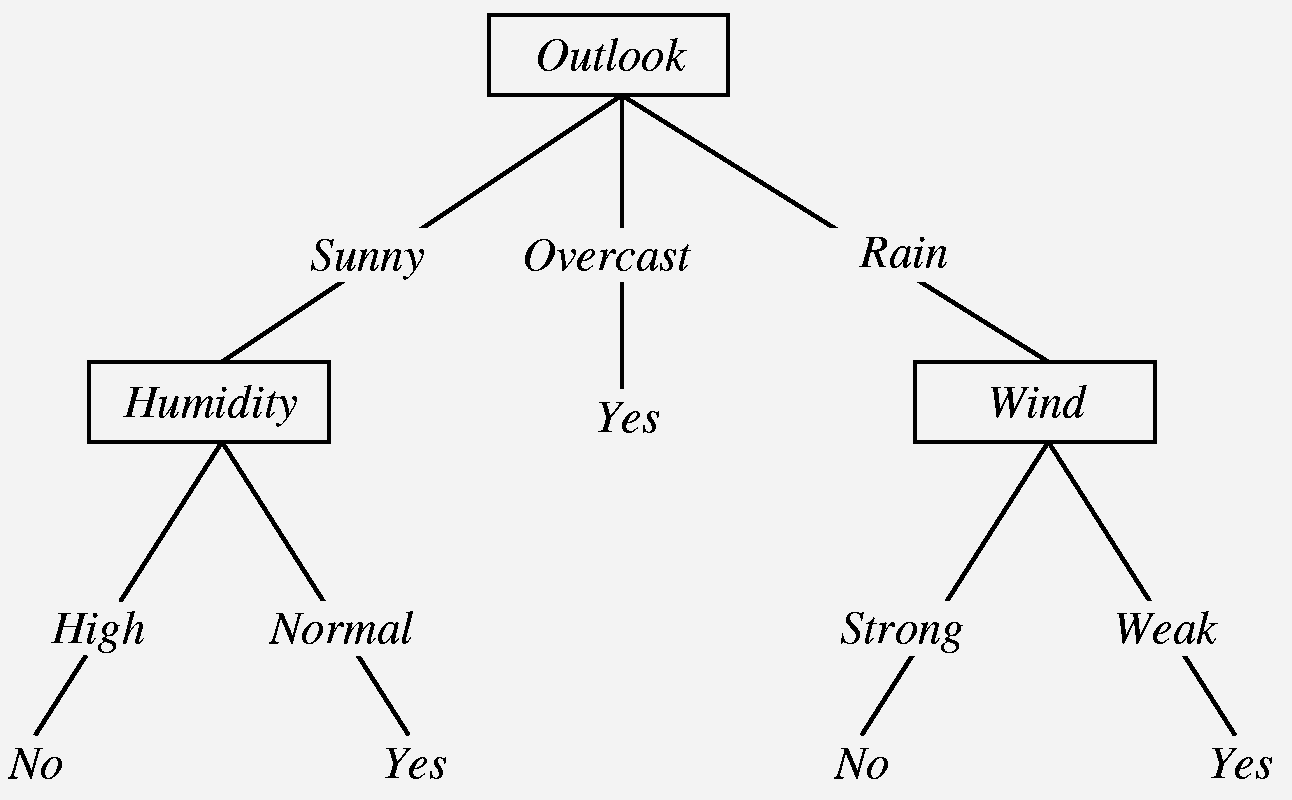
\includegraphics[width=100mm]{figures/ch_03/decision_tree_example.png}
  \caption{Representación de datos en forma de árbol de decisión. \cite{vidal2009decision}}
  \label{fig:3.1}
\end{figure}

Existen varias \emph{implementaciones} de estos árboles, pero aquí veremos una concreta, de las más fáciles de entender, el algoritmo \emph{ID3}. Sus siglas vienen de \emph{Iterative Dichotomiser 3}, \emph{Docotomizador Iterativo 3} en español, creado por Ross Quinlan en \citeyear{quinlan1986induction}, \cite{quinlan1986induction}. A continuación se describe el algoritmo ID3, que crea un árbol para clasificación binaria\footnote{Un problema de clasificación binaria es aquel en el que solo se disponen de dos clases para clasificar las instancias de $\mathcal{D}$, pudiendo ser también una clase y su negación.}, en el cual las dos clases son representadas con $+$, clase positiva, y $-$, clase negativa.

\vspace*{3mm}
\lstset{style=pseudocode}
\begin{lstlisting}
definir id3($ejemplos$, $atributo-objetivo$, $atributos$):
  si todos los $ejemplos$ son positivos:
    devolver un nodo etiquetado con $+$
  si todos los $ejemplos$ son negativos:
    devolver un nodo etiquetado con $-$
  si $atributos$ es vacio:
    devolver un nodo con la etiqueta mas frecuente de $atributo-objetivo$ en $ejemplos$
  en otro caso:
    calcular $A$ como el atributo en $atributos$ que MEJOR CLASIFIQUE $ejemplos$
    crear $arbol$ con $A$ como nodo raiz
    para cada valor $a_{i}$ de $A$:
      crear una rama etiquetada con $a_{i}$
      crear $ejemplos(a_{i})$ como el subconjunto de $ejemplos$ con $A$ igual a $a_{i}$
      si $ejemplos(a_{i})$ es vacio:
        colocar debajo de la rama $a_{i}$ un nodo con la etiqueta mas frecuente de $atributo-objetivo$ en $ejemplos$
      en otro caso:
        colocar debajo de la rama $a_{i}$ el subarbol id3($ejemplos(a_{i})$, $atributo-objetivo$, $atributos - A$)
    devolver $arbol$

id3($\mathcal{D}$, $\mathcal{Y}$, $\mathcal{X}$)
\end{lstlisting}

A la sencillez del algoritmo ID3 solo hay que puntuar lo que significa \emph{atributo que mejor clasifique}. Para ello nos apoyamos en dos conceptos, \emph{entropía} y \emph{ganancia}.

\begin{itemize}
\item[\textbullet]La entropía, $H$, mide la incertidumbre de la clasificación de un conjunto de datos $\mathcal{D}_{i}$:

$$
H(\mathcal{D}_{i})\:=\:-\:\frac{|P_{i}|}{|\mathcal{D}_{i}|}\cdot\log_{2}\frac{|P_{i}|}{|\mathcal{D}_{i}|}\:-\:\frac{|N_{i}|}{|\mathcal{D}_{i}|}\cdot\log_{2}\frac{|N_{i}|}{|\mathcal{D}_{i}|}
$$

\noindent
donde $P_{i}$ y $N_{i}$ son, respectivamente, los conjuntos de ejemplos positivos y negativos de $\mathcal{D}_{i}$.

\item[\textbullet]La ganancia de información es la diferencia de entropía de un conjunto de datos $\mathcal{D}_{i}$ con la que exista después de escoger un atributo $A$ cómo nodo actual en el árbol:

$$
IG(\mathcal{D}_{i},\:A)\:=\:H(\mathcal{D}_{i})\:-\:\sum_{a\:\in\:A}\frac{|\mathcal{D}_{i,\:a}|}{\mathcal{D}_{i}}\cdot H(\mathcal{D}_{i,\:a})
$$

donde $a$ son los distintos valores de la variable $A$, y $\mathcal{D}_{i,\:a} $ es el subconjunto de $\mathcal{D}_{i}$ con $A\:=\:a$.
\end{itemize}

Así que, respondiendo a la pregunta sobre qué significa \emph{atributo que mejor clasifique}, sería un atributo $A$, de entre los existentes, que posee la mayor ganancia de información en el conjunto de ejemplos actuales $\mathcal{D}_{i}$, ($ejemplos$, también en el algoritmo). Otros algoritmos para la creación de árboles de decisión, como el \emph{CART}, miden la \emph{impureza} de los nodos mientras construyen el árbol, utilizando una técnica llamada impureza de Gini. Así, los nodos con menor impureza serán elegidos en cada paso del algoritmo.

Para finalizar, se puede comentar que existen técnicas que mejoran el rendimiento de los algoritmos que crean estos árboles, incluso procesos que mejoran los árboles ya creados, como la $poda$, que devuelve un árbol más pequeño con mejor rendimiento o el mismo árbol en el caso de que no se pueda podar.

\subsection{Máquinas de soporte vectorial} \label{subsec:3.1.2}

Las máquinas de soporte vectorial, \emph{support vector machines} (\emph{SVM}) en inglés, resuelven un problema parecido al de la regresión lineal (subsección \ref{subsec:2.5.3}), buscar un hiperplano. Como diferencia con la regresión, las SVM no buscan un hiperplano que se \emph{ajuste} con el menor error posible a los datos, sino algo bastante opuesto. El objetivo es encontrar el hiperplano que más separe los datos de entrada según su clase de salida, por eso este problema nació como uno de clasificación binaria, siendo actualmente ajustable a clasificación multiclase y a regresión.

Entonces, como premisa de este algoritmo, lo que se busca es que el hiperplano tenga en una lado todo el subconjunto de datos pertenecientes a una clase, por ejemplo $\mathcal{D}_{+}$, y en la otra el de la otra clase, $\mathcal{D}_{-}$, lo que se conoce cómo \emph{separación lineal}. Además se busca que los puntos más cercanos al hiperplano estén separados del mismo la máxima distancia posible, a lo que también se conoce cómo \emph{margen máximo}.

\begin{figure}[ht]
  \centering
  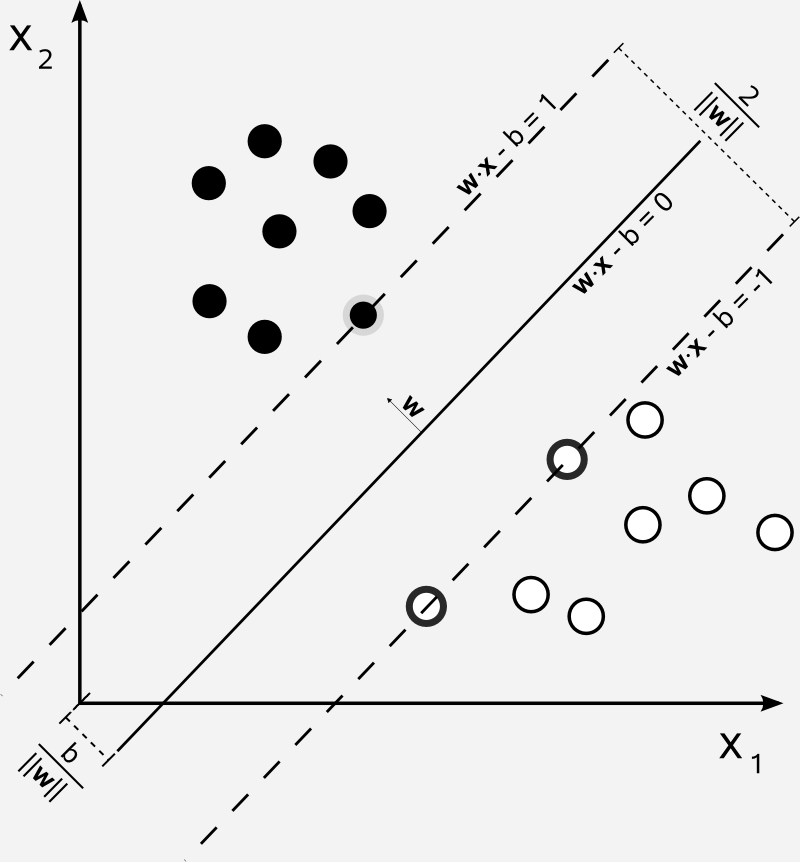
\includegraphics[width=75mm]{figures/ch_03/svm_margin.png}
  \caption{Representación del problema de encontrar el margen máximo para SVM. \cite{wikipedia2014support}}
  \label{fig:3.2}
\end{figure}

Según la figura \ref{fig:3.2}, la recta, o hiperplano, viene representada por:

$$
w \cdot x\:-\:b\:=\:0
$$

\noindent
donde $x$ es el vector con las variables del espacio de entrada, $\mathcal{X}$; $w$ el vector normal al hiperplano con $|w|\:=\:|x|$; y $b$ determina el desplazamiento respecto del origen de coordenadas. Esta recta es la que posee mayor margen, \emph{margen máximo} $=\:\frac{2}{\lVert w \rVert}$, encontrándose en el punto medio de este. Además, las rectas:

$$
w \cdot x\:-\:b\:=\:\pm1
$$

\noindent
serían los límites de dicho margen.

Dados estos parámetros, solo tendríamos que minimizar la norma de $w$, $\lVert w \rVert$, y ajustar el desplazamiento $b$. Una herramienta para solucionar este problema son los \emph{multiplicadores de Lagrange}, una solución con una complejidad relativa mayor a lo que se encuentra en este documento. Con lo estudiado hasta aquí se puede llegar a comprender el funcionamiento general de las máquinas de soporte vectorial, aunque aún pueda surgir alguna que otra pregunta.

Una de estas cuestiones podría ser la siguente: ¿qué ocurre si $\mathcal{D}$ no es linealmente separable? El método más común es aplicar una \emph{función kernel}, la cual transforma $\mathcal{X}$ añadiéndole más atributos, ($\mathcal{X}_{n\:+\:1}$, $\mathcal{X}_{n\:+\:2}$, \dots) para encontrar un hiperplano que separe los datos en ese nuevo espacio de atributos. En la figura \ref{fig:3.3} podemos apreciar un ejemplo de estas transformaciones, donde se mantiene la misma variable en el eje de ordenadas y se muestra una nueva en el de abscisas, consiguiendo una separación totalmente lineal en el conjunto de datos.

\begin{figure}[ht]
  \centering
  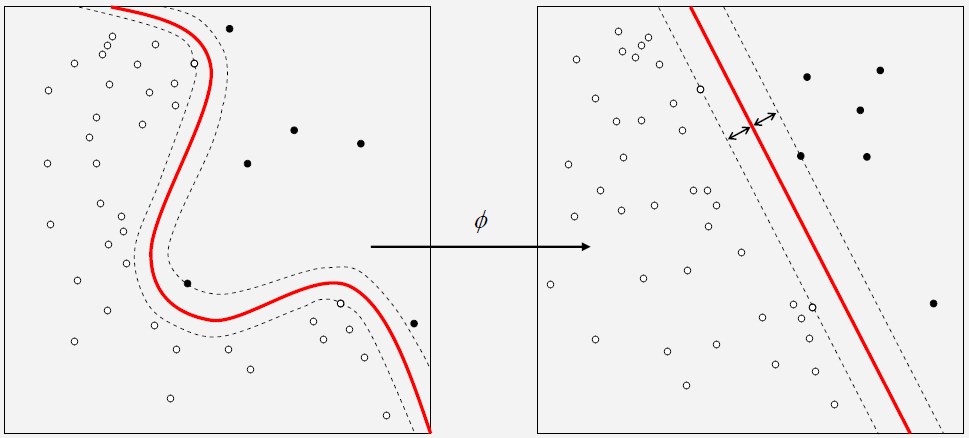
\includegraphics[width=120mm]{figures/ch_03/svm_kernel.png}
  \caption{Representación de un ejemplo de una función kernel para SVM. \cite{wikipedia2014support}}
  \label{fig:3.3}
\end{figure}

\subsection{Redes neuronales artificiales} \label{subsec:3.1.3}

Las redes neuronales artificiales son un modelo de machine learning inspirado en la biología, concretamente en el sistema nervioso central de los animales. Estas simulan una red de neuronas biológicas interconectadas, las cuales son capaces de computar una salida a partir de una señal de entrada, en nuestro caso todo sería instancias de $\mathcal{D}$.

\begin{figure}[ht]
  \centering
  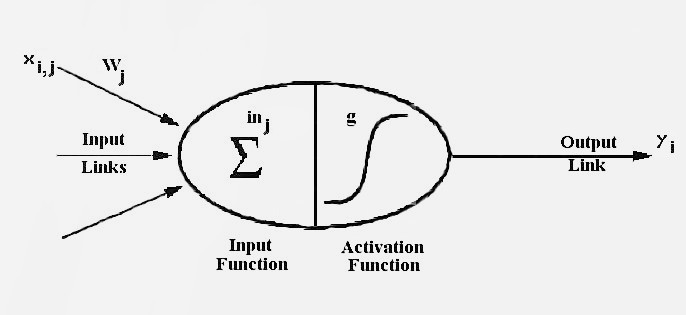
\includegraphics[width=120mm]{figures/ch_03/perceptron_example.jpg}
  \caption{Representación del perceptrón simple. \cite{kendall2001introduction}}
  \label{fig:3.4}
\end{figure}

Para comprender cómo funcionan estas redes, veamos su ejemplo más sencillo, el \emph{perceptrón simple}, mostrado en la figura \ref{fig:3.4}. En este modelo, como en redes más complejas, tendríamos como entradas los valores de las variables de $\mathcal{X}$, que serían procesados para producir una salida, $\mathcal{Y}$, según una \emph{función de activación}. Estos valores de entrada no pasan tal cual a la función de activación, sino que se multiplican por ciertos \emph{pesos}, $w_{j}$, los cuales hay que buscar para proporcionar la salida correcta. Esta búsqueda es el \emph{entrenamiento} de las redes neuronales. Como función de activación, que suele recibir el sumatorio de las entradas, $x_{i,\:j}$, multiplicadas por los pesos, $w_{i}$, se suele escoger una función por partes llamada \emph{umbral}, quedando el perceptrón representado por:

$$
y_{i}\:=\:\left\{{\begin{array}{*{3}{c}}
  1 & & \sum_{j\:=\:0}^{n}\:w_{j}x_{i,\:j}\:\geq\:0 \\
  \\
  -1 & & \textrm{en otro caso}
\end{array}} \right.
$$

\noindent
donde $n$ en este caso no es $|\mathcal{X}|$, sino $|\mathcal{X}|\:+\:1$, con lo cual creamos una nueva entrada $x_{i,\:0}\:=\:-1$ , un valor de sesgo que funciona como el valor de orden $0$ en una ecuación.

Veamos el algoritmo de entrenamiento del perceptrón simple con función de activación umbral, un algoritmo que solo converge si las instancias de $\mathcal{D}$ son \emph{linealmente separables}, dada la simpleza del perceptrón.

\vspace*{3mm}
\lstset{style=pseudocode}
\begin{lstlisting}
definir entrena_perceptron($\mathcal{D}$, $\vec{w}$, $\eta$):
  para cada instancia $(x_{i},\:y_{i})$ en $\mathcal{D}$:
    crear $\vec{x_{i}}\:=\:(-1,\:x_{i,\:1},\:\dots,\:x_{i,\:n\:-\:1})$
    calcular $o\:=\:umbral(\vec{w},\:\vec{x_{i}})$
    para cada $w_{i}$ en $\vec{w}$:
      $w_{i}\:\leftarrow\:w_{i}\:+\:\eta(y_{i}\:-\:o)$
  si $\vec{w}$ no clasifica correctamente todo $\mathcal{D}$:
    entrena_perceptron($\mathcal{D}$, $\vec{w}$, $\eta$)
  en otro caso:
    devolver $\vec{w}$

crear $\vec{w}\:=\:(w_{0},\:w_{1},\:\dots,\:w_{n})$ con valores $w_{i}$ aleatorios
entrena_perceptron($\mathcal{D}$, $\vec{w}$, $\eta$)
\end{lstlisting}

Este proceso, junto a un factor de aprendizaje $\eta$ de valor muy pequeño, $0.1$ aproximadamente, va ajustando los pesos del vector $\vec{w}$, según cuánto se equivoque al predecir $y_{i}$. El algoritmo acaba cuando los pesos son capaces de ajustar correctamente todos los $y_{i}$ de $\mathcal{D}$.

\begin{figure}[ht]
  \centering
  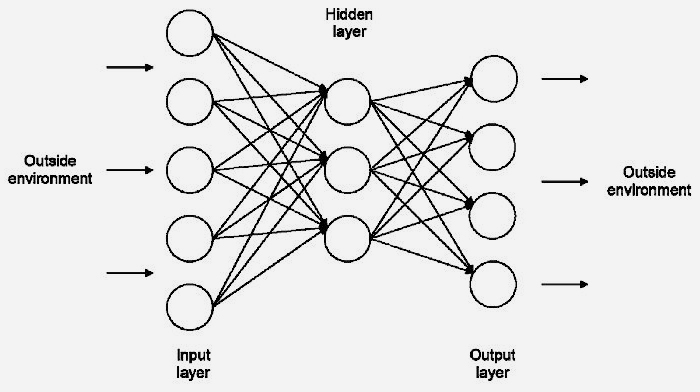
\includegraphics[width=120mm]{figures/ch_03/neural_network_example.jpg}
  \caption{Representación de una red neuronal con una capa oculta sin retroalimentación. \cite{manzi2013from}}
  \label{fig:3.5}
\end{figure}

El perceptrón simple, dada su sencillez, se puede extender a modelos y problemas más complejos, donde las salidas de distintas neuronas funcionan cómo las entradas de otras. Esto llega a crear redes con un número variado de capas de neuronas, donde la primera funciona como capa entrada de los datos y la última como capa de salida, como se muestra en la figura \ref{fig:3.5}. Incluso existen modelos, llamados \emph{con retroalimentación}, en los cuales la salida de una neurona puede funcionar como entrada para ella misma o para algunas de la misma capa o de las capas anteriores. Por estas razones a las redes neuronales artificiales se les llama modelos de \emph{caja negra}, ya que cuando su complejidad aumenta, es muy difícil saber cómo están trabajando las neuronas en su interior después del entrenamiento.

\subsection{Métodos combinados} \label{subsec:3.1.4}

Los llamados en inglés \emph{emsemble methods}, son simplemente varias configuraciones para combinar algoritmos de machine learning, y así proporcionar un mejor resultado. El método más común de esta categoría, el \emph{bootstrap aggregating} o también llamado \emph{bagging}, consiste en crear y entrenar tantos modelos como se deseen, no necesariamente el mismo, de forma que cada uno entrene con un subconjunto distinto de $\mathcal{D}$. Además, a la hora de predecir, cada modelo votará por su solución con igual peso que los demás.

\begin{figure}[ht]
  \centering
  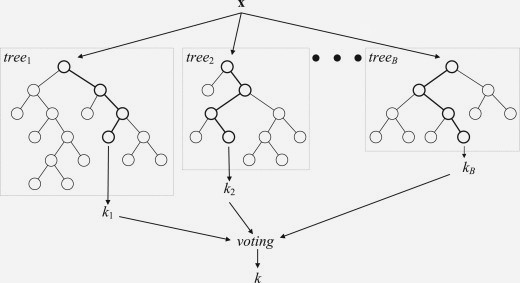
\includegraphics[width=120mm]{figures/ch_03/random_forests_example.jpg}
  \caption{Representación de un random forest. \cite{harmati2014elvarazsolt}}
  \label{fig:3.6}
\end{figure}

Un ejemplo de bagging, con una leve modificación, son los muy usados \emph{Random Forest}, representados en la figura \ref{fig:3.6}. Este \emph{bosque aleatorio} es un conjunto de árboles de decisión, con la peculiaridad de que, cuando cada árbol es creado, sus nodos (atributos) se escogen aleatoriamente y no buscando cuál de ellos sería más conveniente para el subconjunto de datos $\mathcal{D}_{i}$ que está procesando.

\section{Midiendo el rendimiento} \label{sec:3.2}

En esta sección veremos distintas definiciones y técnicas que nos ayudarán a medir distintos tipos de rendimiento en los algoritmos de machine learning, técnicas que no solo se usan tras el aprendizaje sino también durante el mismo proceso.

\subsection{Generalización y sobreaprendizaje} \label{subsec:3.2.1}

Dos términos que a priori pueden sonar confusos son \emph{generalización} y \emph{sobreaprendizaje}, ambos características que un modelo ofrece sobre sus resultados. Podemos pensar que si un modelo ya entrenado se encuentra con una instancia para clasificarla, puede generalizarla, darle un valor muy general y errar en el resultado. O en caso contrario, si el modelo ofrece sobreaprendizaje, habrá aprendido muy bien de los datos, y conseguirá aplicar el resultado casi perfectamente. Pues la realidad es otra, justamente la contraria.

Se dice que un modelo puede generalizar muy bien, cuando se encuentra ante unos datos de entrada poco parecidos con los que ha sido entrenado y, además, produce un buen resultado.

El sobreaprendiazje, \emph{overfitting} en inglés, es cuando el modelo, por varias posibles razones, no es capaz de \textbf{generalizar}, y solo predice correctamente entradas parecidas, o las mismas, a las que aprendió.

La forma en la que se usa el concepto \emph{generalizar} en la descripción de sobreaprendizaje, hace indicar claramente que son términos opuestos. Si un modelo es capaz de generalizar, apenas tendrá sobreaprendizaje, y viceversa.

Las posibles razones del sobreaprendizaje para cierto modelo, incluyendo la elección del algoritmo, van desde tener un bajo número de instancias en los datos de las que aprender, hasta que estos tengan una cantidad de ruido\footnote{El ruido se puede definir cómo la aparición de valores atípicos o erróneos en los datos.} elevada o que el objetivo del modelo sea difícil de alcanzar. La tabla \ref{table:3.1} ofrece una visión muy simple de este párrafo.

\begin{table}[H]
\centering
\colorbox{lightgray}{\begin{tabular}{*{5}{c}}
  Número de instancias & $\uparrow$ & \; & Sobreaprendizaje & $\downarrow$ \\
  Ruido en los datos & $\uparrow$ & \; & Sobreaprendizaje & $\uparrow$ \\
  Dificultad del modelo & $\uparrow$ & \; & Sobreaprendizaje & $\uparrow$
\end{tabular}}
\caption{Posibles razones de sobreaprendizaje en un modelo.}
\label{table:3.1}
\end{table}

En la subsección \emph{\ref{subsec:3.2.3} \nameref{subsec:3.2.3}}, hablaremos brevemente de nuevo sobre el sobreaprendizaje y cómo medirlo, esta vez como \emph{error} que es, y no como un concepto.

\subsection{Validación cruzada} \label{subsec:3.2.2}

Aprender de un conjunto de datos y probar el rendimiento del modelo sobre el mismo conjunto es un error metodológico: el modelo podría haber aprendido perfectamente las instancias con las que fue entrenado y errar complemente en predicciones nuevas. Un grave error de sobreaprendizaje.

Para evitar situaciones como ésta, la técnica más utilizada, llamada \emph{validación cruzada} o \emph{cross-validation} en inglés, consiste en dividir el conjunto en un subconjunto de aprendizaje, $\mathcal{D}_{apren}$, y en otro de validación o prueba, $\mathcal{D}_{val}$. Esto hace que podamos medir el rendimiento del modelo en un conjunto de datos no utilizados en el aprendizaje, y tener así una estimación de cómo se comportará posteriormente con datos reales. Un tamaño muy usado para $\mathcal{D}_{val}$ es utilizar el $10\%$ o el $20\%$ del tamaño total de $\mathcal{D}$, dejando el $90\%$ o el $80\%$ respectivamente para $\mathcal{D}_{apren}$. 

Existen ciertos ajustes para mejorar aún más la medida del rendimiento cuando se utiliza validación cruzada, siendo los más usados el llamado \emph{$k$-fold} y la \emph{estratificación}. $k$-fold consiste en dividir el conjunto de datos en $k$ subconjuntos de igual tamaño. Usando $k$-fold se necesitan realizar $k$ entrenamientos para medir el rendimiento, en los cuales $\mathcal{D}_{val}$ se irá alternando entre cada \emph{fold} creado, dejando el resto de particiones como un solo $\mathcal{D}_{val}$, como se muestra en la figura \ref{fig:3.7}. Unos valores para $k$ bastante utilizados son $5$ y $10$.

\begin{figure}[H]
  \centering
  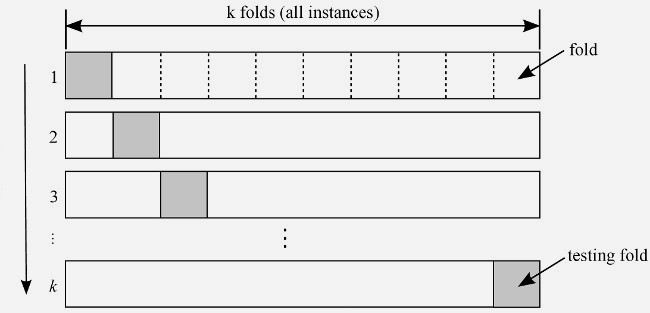
\includegraphics[width=120mm]{figures/ch_03/k_fold_example.jpg}
  \caption{Representación de $\mathcal{D}$ para validación cruzada con $k$-fold. \cite{ekroth2012intro}}
  \label{fig:3.7}
\end{figure}

La estratificación es una variación mínima del $k$-fold, donde cada subconjunto de los $k$ creados contiene aproximadamente el mismo porcentaje de instancias de cada clase, consiguiendo más homogeneidad en las medidas del aprendizaje y de la validación.

\subsection{Error} \label{subsec:3.2.3}

Una vez aprendidos conceptos previos como generalización, sobreaprendizaje y validación cruzada, podemos empezar a medir el rendimiento. Cómo medir el rendimiento depende del tipo de problema al que nos enfrentemos. Intentar medirlo en problemas de clustering es algo inusual, ya que no tenemos una solución correcta de antemano para comparar los resultados obtenidos. Así que el problema de medir el rendimiento se reduce a casos de clasificación y regresión. Comencemos con este último.

En problemas de regresión, la forma de medir el rendimiento es medir el error cometido al predecir. Se pueden utilizar técnicas como el error absoluto medio, \emph{mean absolute error} (\emph{MAE}) en inglés, o el error cuadrático medio, \emph{mean squared error} (\emph{MSE}) en inglés.

El error absoluto medio se define cómo el promedio de los errores en las predicciones. El error en una predicción viene dado por

$$
E\:=\:g(x_{i})\:-\:f(x_{i})
$$

\noindent
siendo $x_{i}$ una instancia de $\mathcal{D}$, $f$ la función ideal de predicción y $g$ nuestra hipótesis para predecir. Así el MAE quedaría como:

$$
MAE\:=\:\frac{\sum_{i\:=\:1}^{|\mathcal{X}|}|g(x_{i})\:-\:f(x_{i})|}{N}
$$

El error cuadrático medio se corresponde con la media de los errores al cuadrado, tomando valores elevados cuando existen errores grandes, una forma de castigar más al error:

$$
MSE\:=\:\frac{\sum_{i\:=\:1}^{|\mathcal{X}|}(g(x_{i})\:-\:f(x_{i}))^{2}}{N}
$$

Escoger uno u otro depende del tipo de datos encontrado en el espacio de salida, $\mathcal(Y)$, y en el modelo utilizado.

Si queremos mejorar el resultado de la regresión a partir de la medida del error, necesitamos acercarnos a ciertas técnicas, siendo una de estas la compensación entre sesgo y varianza, o \emph{bias-variance trade-off} en inglés. El sesgo se puede describir como cuánto de impreciso ha sido el modelo, y la varianza como una medida de la sensibilidad del modelo a pequeños cambios irrelevantes en $\mathcal{D}$. Otra percepción importante del sesgo es compararlo con uno de los casos de sobreaprendizaje, en el que hayamos \emph{sesgado} los datos a solo los que cumplan ciertos requerimientos, perdiendo generalización para instancias reales.

Ambos términos, sesgo y varianza, se pueden extraer matemáticamente a partir del error, pero lo interesante de ellos es saber cómo detectarlos y compensarlos para mejorar el rendimiento del modelo, ya que lo ideal es no tener sesgo y varianza y por lo tanto no tener error. Ya que esto es una tarea casi imposible tenemos que ajustar uno de ellos, sabiendo que si mejoramos uno, empeoraremos el otro. Para esta tarea se utilizan las curvas de aprendizaje.

\begin{figure}[ht]
  \centering
  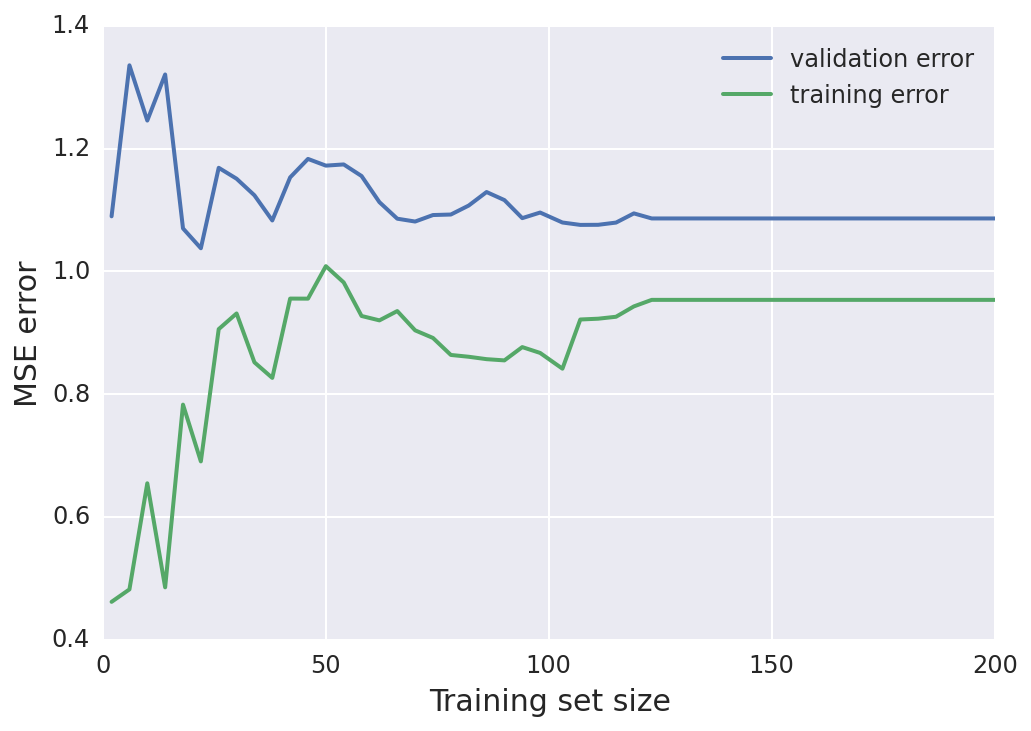
\includegraphics[width=120mm]{figures/ch_03/learning_curve_example.png}
  \caption{Representación de una curva de aprendizaje.}
  \label{fig:3.8}
\end{figure}

Las curvas de aprendizaje (figura \ref{fig:3.8}), representan el error en el aprendizaje y en la predicción conforme el tamaño de $\mathcal{D}$ aumenta. La validación cruzada juega aquí un papel importante, ya que podemos obtener el error de predicción antes de enfrentarnos a problemas reales, utilizando un conjunto de validación y obteniendo su error.

En estas curvas, podemos detectar un \emph{sesgo alto} si el error de validación decrece al comienzo de la gráfica pero se establece a valores más altos conforme el tamaño de $\mathcal{D}$ aumenta. Una \emph{varianza alta} se puede detectar si encontramos una diferencia bastante importante entre la representación de ambos errores al final de la gráfica.

Si nos encontramos en el caso de que sufrimos de sesgo alto, podemos arreglarlo creando más atributos y añadiéndolos a $\mathcal{X}$, o cambiar el modelo a una versión más compleja del mismo o a otro diferente con una complejidad mayor.

Si sufrimos de varianza alta significa que nuestro modelo es muy complejo. Para solventar este problema podemos añadir más instancias a $\emph{D}$ o disminuir la complejidad del modelo.

Visto esto podemos afirmar lo que se comentó anteriormente, solo se puede tratar de mejorar uno de los atributos del modelo.

\subsection{Exactitud} \label{subsec:3.2.4}

Existen casos donde el error no se puede calcular a través de funciones como el error cuadrático medio. Estos casos son los problemas de clasificación, donde no tenemos una salida cuantitativa, sino cualitativa, teniendo que definir una nueva medida del rendimiento. Una de las medidas es la simple exactitud, \emph{accuracy} en inglés, que mide la proporción de instancias bien clasificadas, un valor entre $0$ y $1$.

Algunos autores intentan obtener una medida del error en la clasificación, aunque ninguna de ellas está extendida, aunque en \cite{richert2013building} proponen una media del error:

$$
E\:=\:1\:-\:exactitud
$$

\noindent
no siendo habitual su uso.

Existen un par métodos para extraer algo de más información del rendimiento \textbf{de cada clase a predecir} en un problema de clasificación. Estos son la obtención de la precisión/exhaustividad, \emph{precision/recall} (\emph{P/R}) en inglés, y de la característica operativa del receptor, \emph{receiver operating characteristic} (\emph{ROC}) también en inglés. Pero antes se necesita definir ciertos términos.

En la tabla \ref{table:3.2} vemos las expresiones verdadero positivo, verdadero negativo, falso positivo y falso negativo, abreviados por TP, TN, FN y FP, \emph{true} y \emph{false} en inglés. Los términos positivo y negativo se refieren a la predicción del clasificador \emph{para la clase que se está evaluando}, y los términos falso y negativo se refieren a si la predicción es correcta o no evaluándola con la salida de la instancia en $\mathcal{D}$.

\begin{table}[ht]
\centering
\colorbox{lightgray}{\begin{tabular}{*{4}{c}}
  & & \multicolumn{2}{c}{\textbf{Predicción}} \\
  & & \textit{Positivo} & \textit{Negativo} \\
  \textbf{Clase} & \textit{Positivo} & Verdadero positivo (TP) & Falso negativo (FN) \\
  \textbf{real} & \textit{Negativo} & Falso negativo (FN) & Verdadero negativo (TN)
\end{tabular}}
\caption{Descripción de resultados para un problema de clasificación.}
\label{table:3.2}
\end{table}

Para la medida precisión/exhaustividad, P/R, tenemos que:

$$
precicsion\:=\:\frac{TP}{TP\:+\:FP}
$$

\noindent
y

$$
recall\:=\:\frac{TP}{TP\:+\:FN}
$$

\noindent
tomando los valores de TP, FP y FN por la cantidad total de ellos en la clase que se está evaluando. Así, una precisión de $1.0$ significa que cada instancia clasificada como perteneciente a una clase $C$ verdaderamente pertenecía a $C$, sin decir nada del número de instancias de $C$ que no fueron clasificadas correctamente. Y un valor de $1.0$ para la exhaustividad, recall, significa que cada instancia de la clase $C$ fue clasificada correctamente, sin decir cuántas otras instancias se clasificaron incorrectamente como pertenecientes a $C$.

\begin{figure}[ht]
  \centering
  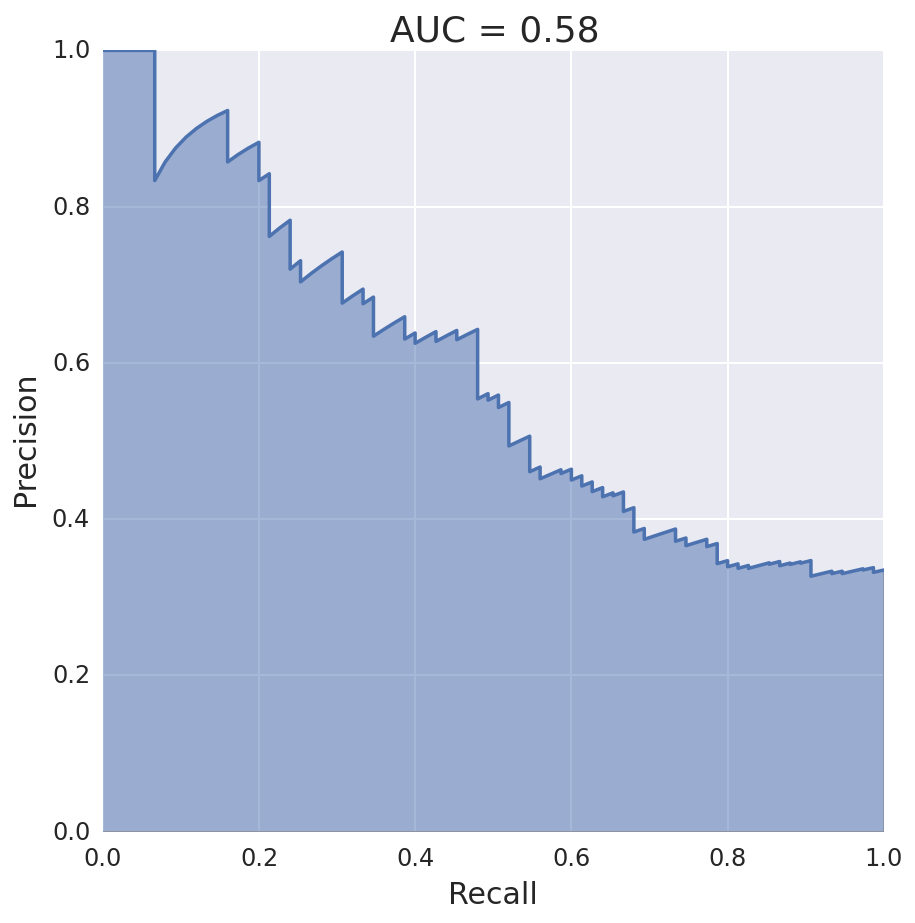
\includegraphics[width=100mm]{figures/ch_03/pr_example.png}
  \caption{Representación del área bajo la curva para medidas de P/R.}
  \label{fig:3.9}
\end{figure}

Estos dos valores, precisión y exhaustividad, se suelen representar en una gráfica (figura \ref{fig:3.9}), describiendo una curva definida por pares de estos valores. Algunos algoritmos utilizan un umbral probabilístico para decir si una instancia pertenece a una clase en cuestión o no. Ajustando este umbral se pueden obtener estos pares de valores, que van de $0$ a $1$ para ambos. Para aquellos algoritmos que no ofrecen este umbral, existen métodos para obtenerlos, por ejemplo, en \cite{wu2004probability} se describe un método para las máquinas de soporte vectorial.

Esta representación es simplemente un paso extra para visualizar una medida implícita en los valores de precisión y exhaustividad, que es el área bajo la curva de estos valores, donde siempre se prefieren áreas grandes, cercanas a $1$. Además, el objetivo final de estas curvas es disponer de una representación donde con un vistazo se puedan localizar posibles problemas en la precisión y la exhaustividad, conociendo siempre la definición de éstas.

Existe un método análogo a éste, la obtención de la característica operativa del receptor, ROC. En ella se necesitan las proporciones de los verdaderos positivos y la de los falsos positivos:

$$
TPR\:=\:\frac{TP}{TP\:+\:FN}
$$

\noindent
y

$$
FPR\:=\:\frac{FP}{FP\:+\:TN}
$$

\begin{figure}[ht]
  \centering
  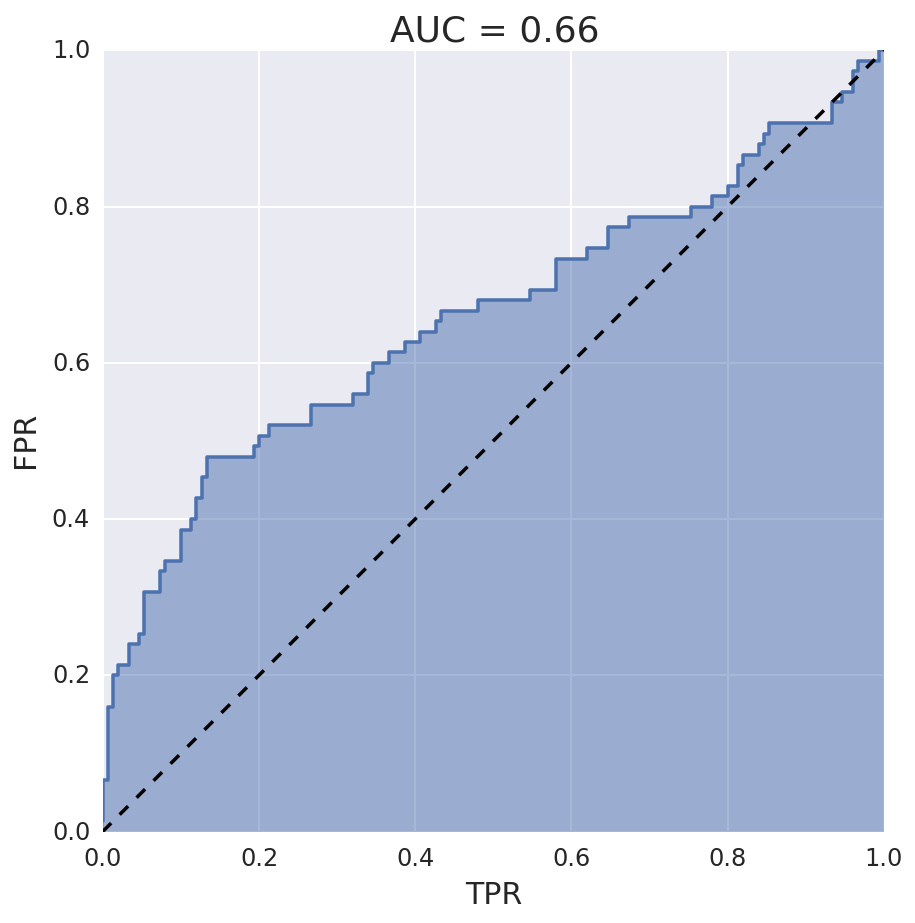
\includegraphics[width=100mm]{figures/ch_03/roc_example.png}
  \caption{Representación del área bajo la curva para medidas de ROC.}
  \label{fig:3.10}
\end{figure}

Podemos observar que TPR es exactamente la exhaustividad de la curva P/R, quedando por definir FPR. Así, un FPR de $1.0$ significa que cada instancia clasificada como perteneciente a una clase $C$ no pertenece a $C$, sin decir cuántas no fueron clasificadas como $C$ cuando no pertenecían a $C$. Además también podemos obtener el área bajo la curva (figura \ref{fig:3.10}), donde también se prefieren valores cercanos a $1$.

Hemos obtenido tres formas de medir el rendimiento en los clasificadores, la exactitud y el área bajo de la curva de P/R y ROC. Quedando la exactitud cómo una medida general y simple, tenemos que diferenciar entre las dos restantes, que son más robustas. P/R se suele utilizar en clasificadores binarios, donde una de las dos clases es más importante que la otra, y por lo tanto esta medida solo se practicaría en la clase principal. ROC se suele utilizar para medir el rendimiento de cada clase, tanto en clasificadores binarios como multiclase, dando además una mejor impresión de cómo se comporta el modelo en general.

Por último, existe otro método llamado \emph{matrices de confusión}, que permiten observar qué clases se clasifican incorrectamente, y además ver con qué clases son confundidas cuando no lo hacen. En estas matrices las filas indican las clases a las que verdaderamente pertenecen las instancias, y las columnas nos muestran cómo se han predicho estas instancias.

\begin{table}[ht]
\centering
\colorbox{lightgray}{\begin{tabular}{*{5}{c}}
  & & \multicolumn{3}{c}{\textbf{Predicción}} \\
  & & \textit{A} & \textit{B} & \textit{C} \\
  \textbf{Clase} & \textit{A} & 5 & 3 & 0 \\
  & \textit{B} & 2 & 3 & 1 \\
  \textbf{real} & \textit{C} & 0 & 2 & 11
\end{tabular}}
\caption{Ejemplo de una matriz de confusión.}
\label{table:3.3}
\end{table}

En la tabla \ref{table:3.3} vemos un ejemplo de estas matrices, donde por ejemplo, de las $8$ instancias de la clase $A$, $5$ se han clasificado correctamente y $3$ incorrectamente como pertenecientes a $B$.

Una forma muy útil de representar estas matrices cuando tenemos un gran número de instancias en $\mathcal{D}$ es utilizar una visualización donde, en lugar de números, se utiliza una gama de colores (figura \ref{fig:3.11}), intentando denotar por colores más oscuros a los números mayores y viceversa. Lo que se busca en un modelo es que la diagonal principal sea lo más oscura posible, así todas las clases se clasificarían de una manera bastante correcta.

\begin{figure}[H]
  \centering
  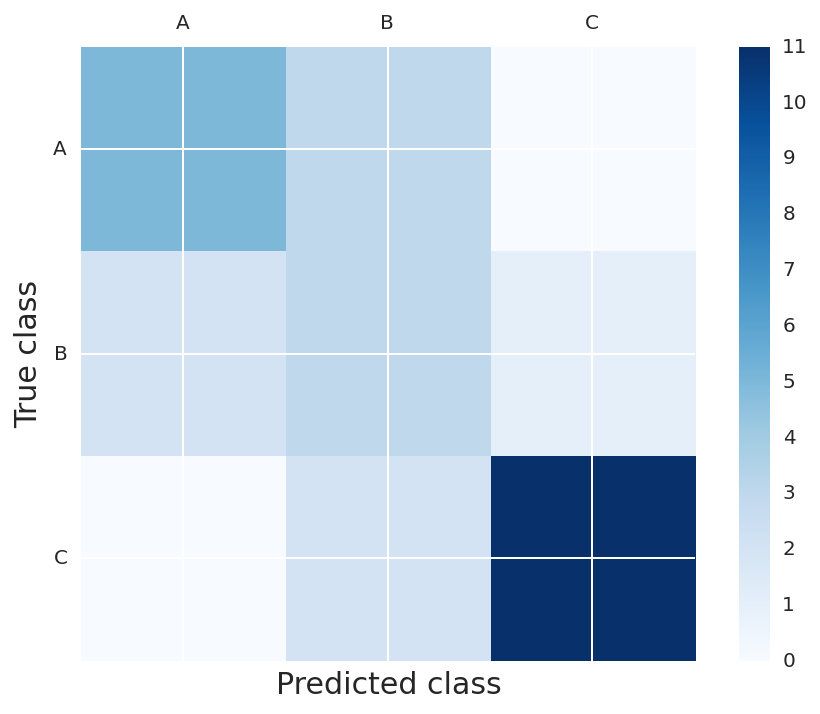
\includegraphics[width=100mm]{figures/ch_03/confusion_matrix_example.png}
  \caption{Ejemplo de una visualización por colores de una matriz de confusión.}
  \label{fig:3.11}
\end{figure}

\section{Reducción de la dimensionalidad} \label{sec:3.3}

Para reducir el error se han comentado, entre varias más, un par de técnicas, como la creación de nuevos atributos, como vimos en la subsección \ref{subsec:2.2.1}, o la eliminación de algunos de éstos. Un método para saber cuáles de los atributos podemos eliminar es conocer la \emph{información mutua} de pares de estos atributos.

La información mutua se define como:

$$
I(\mathcal{X}_{i};\:\mathcal{X}_{j})\:=\:\sum_{x_{i}\in\mathcal{X}_{i}}\sum_{x_{j}\in\mathcal{X}_{j}}p(x_{i},\:x_{j})\:\log_{2}\frac{p(x_{i},\:x_{j})}{p(x_{i})p(x_{j})}
$$

\noindent
siendo $p$ la distribución de probabilidad marginal de cada variable. Pero para poder operar mejor con la información mutua, lo ideal es restringirla al intervalo $[0,\:1]$. Para eso, definimos la \emph{información mutua normalizada} como:

$$
NI(\mathcal{X}_{i};\:\mathcal{X}_{j})\:=\:\frac{I(\mathcal{X}_{i};\:\mathcal{X}_{j})}{H(\mathcal{X}_{i})\:+\:H(\mathcal{X}_{j})}
$$

Siendo $H$ la \emph{entropía de la información} de cada variable. Esta entropía se puede definir como la incertidumbre de la variable. En una definición más formal se puede ver como el valor medio ponderado por la cantidad de información de cada valor único de la variable, también representado por la siguiente función:

$$
H(\mathcal{X}_{i})\:=\:-\sum_{j}p(x_{i,\:j})\:log_{2}p(x_{i,\:j})
$$

\noindent
con $p$ como la función de probabilidad de la variable $\mathcal{X}_{i}$ para cierto valor $x_{i,\:j}$.

Cuando se obtengan estos valores de la información mutua normalizada, $NI$, se podrán eliminar del espacio de entrada, $\mathcal{X}$, aquellas variables que aparezcan repetidamente con valores altos. En la figura \ref{fig:3.12} podemos ver cuatro ejemplos de esta medida, pudiendo determinar que las variables están muy relacionadas, a través cierta cierta función, cuando estas poseen un valor de $NI\:\geq\:2$. En el que caso de que tuviéramos $\mathcal{X}_{i}\:=\:\mathcal{X}_{j}$, la información mutua normalizada, $NI$, sería $1$.

\begin{figure}[H]
  \centering
  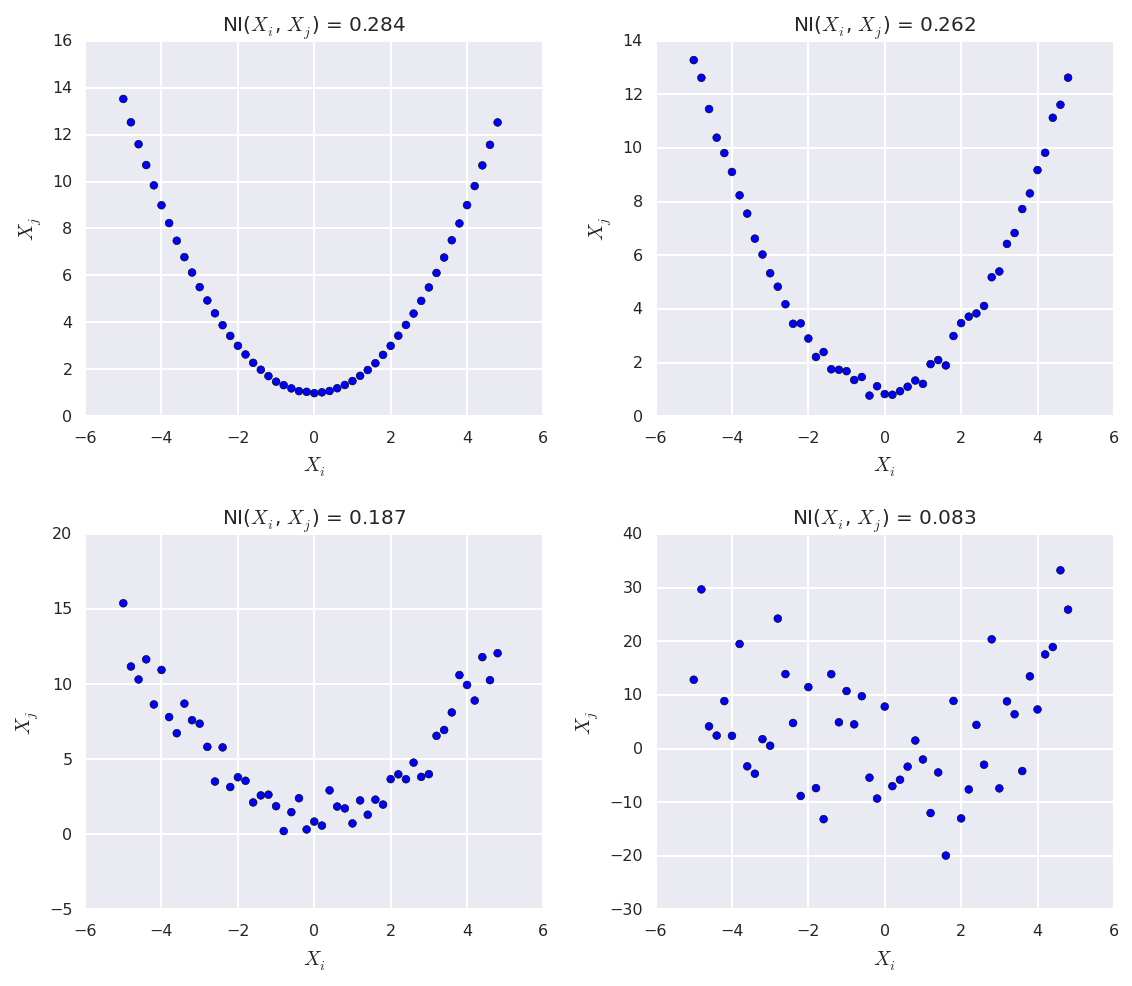
\includegraphics[width=100mm]{figures/ch_03/mutual_information_example.png}
  \caption{Representación de cuatro ejemplos de información mutua normalizada.}
  \label{fig:3.12}
\end{figure}

\section{Metodología} \label{sec:3.4}

Para finalizar con los fundamentos teóricos del aprendizaje automático, tan solo falta estudiar una \emph{metodología} para saber cómo atacar un problema de machine learning. Una simple metodología consiste en seguir una serie de pasos como los que veremos a continuación, teniendo que repetir alguno si se consiguen resultados insatisfactorios:

\begin{enumerate}[label=\textbf{\arabic*.},start=1]
  \item \textbf{Obtener los datos.} En este paso, aparte de conseguir el dataset necesario, $\mathcal{D}$, se tendrá que elegir el objetivo del problema, si es que no se tiene de antemano.
  
  \item \textbf{Seleccionar el modelo.} Aquí se debe escoger qué algoritmo se utilizará. Una forma de resolver esta tarea es visualizar cada variable del espacio de entrada, $\mathcal{X}$, respecto a la/s de salida/s, $\mathcal{Y}$, para saber cómo se relacionan los datos. Así se podrá escoger mejor el algoritmo a utilizar, conociendo cómo funcionan cada uno de ellos pero sobretodo a través de la experiencia personal y el \emph{know-how}.
  
  \item \textbf{Preparar los datos.} Una vez seleccionado el modelo a utilizar, se puede mejorar el estado de los datos para facilitar el aprendizaje al modelo, por ejemplo, limpiado el ruido o eliminando variables cuya información ya esté presente en otras.
  
  \item \textbf{Entrenar y medir el rendimiento.} Una vez preparado todo se puede entrenar el algoritmo y evaluar su resultado. Si éste no nos conviene se puede proceder a repetir los pasos \textbf{2} y \textbf{3}, según lo visto en la sección \ref{sec:3.2}.
\end{enumerate}

\section{Conclusiones} \label{sec:3.5}

Hasta aquí, hemos estudiado parte de los fundamentos teóricos del machine learning, necesarios para poder empezar a trabajar por nosotros mismos. Como detalle personal, estos fundamentos fueron obtenidos durante la lectura y \emph{práctica} de los textos mencionados en la sección \ref{sec:1.2}, de manera que podía ver la utilidad de lo que iba aprendiendo mientras lo estudiaba.

A continuación, veremos dos capítulos donde se verá un resultado pragmático de lo aprendido.
